\newread\synthetichundredusfile%

\newcommand{\IfNonemptySyntheticHundredUsFile}[3]{%
    \IfFileExists{#1}{%
        \openin\synthetichundredusfile=#1
        \ifeof\synthetichundredusfile%
            \closein\synthetichundredusfile%
            #3%
        \else
            \closein\synthetichundredusfile%
            #2%
        \fi
    }{%
        #3%
    }%
}

\newcommand{\SyntheticHundredUsPlot}[3]{%
    \IfNonemptySyntheticHundredUsFile{#3}{%
        \addplot+[#1]
        table [#2, col sep=comma] {#3};
    }{}%
}

\newcommand{\SyntheticHundredUsSchedsimPlot}[1]{%
    \SyntheticHundredUsPlot{mark=none, solid, cLightBlue}{x expr=\thisrow{Req/time_unit} * 10000, y expr=\thisrow{99th (us)} / 10}{data/schedsim/single_queue/FIFO_1000_20_80_#1.csv}%
}

\newcommand{\SyntheticHundredUsYAxisStyle}{%
    scaled y ticks=false,
    ytick={200, 400, 600, 800, 1000},
    yticklabel style={
        /pgf/number format/fixed,
        /pgf/number format/precision=0,
    }%
}

\newcommand{\SyntheticHundredUsPanelWidth}{5.69cm}

\newcommand{\SyntheticHundredUsCommonAxis}{%
    xlabel={Load (KQPS)},
    xmin=0,
    xmax=200,
    ymin=0,
    ymax=1000,
    enlarge y limits=false,
    restrict x to domain*=0:5E9,
    restrict y to domain*=0:1E4,
    \SyntheticHundredUsYAxisStyle,
    axis y line=left,
    axis x line=bottom,
    height=3.9cm,
    width=6.5cm,
    legend cell align=left%
}

\begin{figure*}[!t]
    \centering
    \captionsetup[subfigure]{justification=centering,singlelinecheck=false,width=\SyntheticHundredUsPanelWidth}
    \begin{minipage}{\linewidth}
        \centering
        \begin{subfigure}[b]{\SyntheticHundredUsPanelWidth}
            \centering
            \begin{tikzpicture}[scale=0.875, transform shape, trim axis left, trim axis right]
                \begin{axis}[
                    \SyntheticHundredUsCommonAxis,
                    ylabel={Latency (\si{\micro\second})},
                    legend style={
                        draw=none,
                        font=\footnotesize,
                        anchor=south,
                        at={(0.95, 1.15)},
                        legend columns=2,
                        /tikz/every even column/.append style={column sep=0.7cm},
                    },
                ]
                    \addlegendimage{partitionStyle}
                    \addlegendentry{TCP-CP}

                    \addlegendimage{kcmStyle}
                    \addlegendentry{KCM}

                    \SyntheticHundredUsPlot{workerPoolStyle, x filter/.code={\IfStrEq{\thisrow{dist_config}}{fixed}{}{\def\pgfmathresult{}}}}{x expr=\thisrow{load_pool(QPS)} / 1000, y=latency_pool}{data/synthetic_20_100us.csv}
                    \SyntheticHundredUsPlot{partitionStyle, x filter/.code={\IfStrEq{\thisrow{dist_config}}{fixed}{}{\def\pgfmathresult{}}}}{x expr=\thisrow{load_partition(QPS)} / 1000, y=latency_partition}{data/synthetic_20_100us.csv}
                    \SyntheticHundredUsPlot{floatingStyle, x filter/.code={\IfStrEq{\thisrow{dist_config}}{fixed}{}{\def\pgfmathresult{}}}}{x expr=\thisrow{load_floating(QPS)} / 1000, y=latency_floating}{data/synthetic_20_100us.csv}
                    \SyntheticHundredUsPlot{kcmStyle, x filter/.code={\IfStrEq{\thisrow{dist_config}}{fixed}{}{\def\pgfmathresult{}}}}{x expr=\thisrow{load_kcm_floating(QPS)} / 1000, y=latency_kcm_floating}{data/synthetic_20_100us.csv}
                    \SyntheticHundredUsPlot{rakaiaStyle, x filter/.code={\IfStrEq{\thisrow{dist_config}}{fixed}{}{\def\pgfmathresult{}}}}{x expr=\thisrow{load_rakaia(QPS)} / 1000, y=latency_rakaia}{data/synthetic_20_100us.csv}
                    \SyntheticHundredUsSchedsimPlot{d}
                \end{axis}
            \end{tikzpicture}
            \caption{\add{Fixed (20 connections).}}
        \end{subfigure}
        \hfill
        \begin{subfigure}[b]{\SyntheticHundredUsPanelWidth}
            \centering
            \begin{tikzpicture}[scale=0.875, transform shape, trim axis left, trim axis right]
                \begin{axis}[
                    \SyntheticHundredUsCommonAxis,
                    ylabel style={opacity=0},
                    ylabel={\phantom{Latency}},
                    legend style={
                        draw=none,
                        font=\footnotesize,
                        anchor=south,
                        at={(0.60, 1.15)},
                        legend columns=2,
                        /tikz/every even column/.append style={column sep=0.7cm},
                    },
                ]
                    \addlegendimage{floatingStyle}
                    \addlegendentry{TCP-CS}

                    \addlegendimage{workerPoolStyle}
                    \addlegendentry{Worker Pool}

                    \SyntheticHundredUsPlot{workerPoolStyle, x filter/.code={\IfStrEq{\thisrow{dist_config}}{exponential}{}{\def\pgfmathresult{}}}}{x expr=\thisrow{load_pool(QPS)} / 1000, y=latency_pool}{data/synthetic_20_100us.csv}
                    \SyntheticHundredUsPlot{rakaiaStyle, x filter/.code={\IfStrEq{\thisrow{dist_config}}{exponential}{}{\def\pgfmathresult{}}}}{x expr=\thisrow{load_rakaia(QPS)} / 1000, y=latency_rakaia}{data/synthetic_20_100us.csv}
                    \SyntheticHundredUsPlot{partitionStyle, x filter/.code={\IfStrEq{\thisrow{dist_config}}{exponential}{}{\def\pgfmathresult{}}}}{x expr=\thisrow{load_partition(QPS)} / 1000, y=latency_partition}{data/synthetic_20_100us.csv}
                    \SyntheticHundredUsPlot{floatingStyle, x filter/.code={\IfStrEq{\thisrow{dist_config}}{exponential}{}{\def\pgfmathresult{}}}}{x expr=\thisrow{load_floating(QPS)} / 1000, y=latency_floating}{data/synthetic_20_100us.csv}
                    \SyntheticHundredUsPlot{kcmStyle, x filter/.code={\IfStrEq{\thisrow{dist_config}}{exponential}{}{\def\pgfmathresult{}}}}{x expr=\thisrow{load_kcm_floating(QPS)} / 1000, y=latency_kcm_floating}{data/synthetic_20_100us.csv}
                    \SyntheticHundredUsSchedsimPlot{m}
                \end{axis}
            \end{tikzpicture}
            \caption{\add{Exponential (20 connections).}}
        \end{subfigure}
        \hfill
        \begin{subfigure}[b]{\SyntheticHundredUsPanelWidth}
            \centering
            \begin{tikzpicture}[scale=0.875, transform shape, trim axis left, trim axis right]
                \begin{axis}[
                    \SyntheticHundredUsCommonAxis,
                    ylabel style={opacity=0},
                    ylabel={\phantom{Latency}},
                    legend style={
                        draw=none,
                        font=\footnotesize,
                        anchor=south,
                        at={(0.20, 1.15)},
                        legend columns=2,
                        /tikz/every even column/.append style={column sep=0.7cm},
                    },
                ]
                    \addlegendimage{rakaiaStyle}
                    \addlegendentry{\system}

                    \addlegendimage{mark=none, cLightBlue}
                    \addlegendentry{MS}

                    \SyntheticHundredUsPlot{workerPoolStyle, x filter/.code={\IfStrEq{\thisrow{dist_config}}{bimodal}{}{\def\pgfmathresult{}}}}{x expr=\thisrow{load_pool(QPS)} / 1000, y=latency_pool}{data/synthetic_20_100us.csv}
                    \SyntheticHundredUsPlot{rakaiaStyle, x filter/.code={\IfStrEq{\thisrow{dist_config}}{bimodal}{}{\def\pgfmathresult{}}}}{x expr=\thisrow{load_rakaia(QPS)} / 1000, y=latency_rakaia}{data/synthetic_20_100us.csv}
                    \SyntheticHundredUsPlot{partitionStyle, x filter/.code={\IfStrEq{\thisrow{dist_config}}{bimodal}{}{\def\pgfmathresult{}}}}{x expr=\thisrow{load_partition(QPS)} / 1000, y=latency_partition}{data/synthetic_20_100us.csv}
                    \SyntheticHundredUsPlot{floatingStyle, x filter/.code={\IfStrEq{\thisrow{dist_config}}{bimodal}{}{\def\pgfmathresult{}}}}{x expr=\thisrow{load_floating(QPS)} / 1000, y=latency_floating}{data/synthetic_20_100us.csv}
                    \SyntheticHundredUsPlot{kcmStyle, x filter/.code={\IfStrEq{\thisrow{dist_config}}{bimodal}{}{\def\pgfmathresult{}}}}{x expr=\thisrow{load_kcm_floating(QPS)} / 1000, y=latency_kcm_floating}{data/synthetic_20_100us.csv}
                    \SyntheticHundredUsSchedsimPlot{b}
                \end{axis}
            \end{tikzpicture}
            \caption{\add{Bimodal (20 connections).}}
        \end{subfigure}
    \end{minipage}

    \begin{minipage}{\linewidth}
        \centering
        \begin{subfigure}[b]{\SyntheticHundredUsPanelWidth}
            \centering
            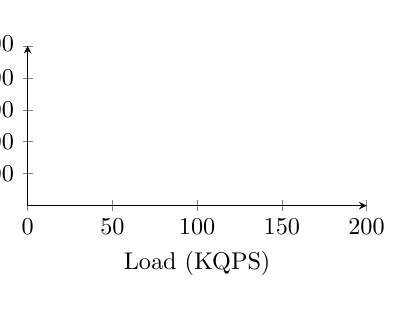
\begin{tikzpicture}[scale=0.875, transform shape, trim axis left, trim axis right]
                \begin{axis}[
                    \SyntheticHundredUsCommonAxis,
                    ylabel={Latency (\si{\micro\second})},
                    legend style={
                        draw=none,
                        font=\footnotesize,
                        anchor=north east,
                        at={(0.50, 0.99)},
                    },
                ]
                    \SyntheticHundredUsPlot{workerPoolStyle, x filter/.code={\IfStrEq{\thisrow{dist_config}}{fixed}{}{\def\pgfmathresult{}}}}{x expr=\thisrow{load_pool(QPS)} / 1000, y=latency_pool}{data/synthetic_80_100us.csv}
                    \SyntheticHundredUsPlot{partitionStyle, x filter/.code={\IfStrEq{\thisrow{dist_config}}{fixed}{}{\def\pgfmathresult{}}}}{x expr=\thisrow{load_partition(QPS)} / 1000, y=latency_partition}{data/synthetic_80_100us.csv}
                    \SyntheticHundredUsPlot{floatingStyle, x filter/.code={\IfStrEq{\thisrow{dist_config}}{fixed}{}{\def\pgfmathresult{}}}}{x expr=\thisrow{load_floating(QPS)} / 1000, y=latency_floating}{data/synthetic_80_100us.csv}
                    \SyntheticHundredUsPlot{kcmStyle, x filter/.code={\IfStrEq{\thisrow{dist_config}}{fixed}{}{\def\pgfmathresult{}}}}{x expr=\thisrow{load_kcm_floating(QPS)} / 1000, y=latency_kcm_floating}{data/synthetic_80_100us.csv}
                    \SyntheticHundredUsPlot{rakaiaStyle, x filter/.code={\IfStrEq{\thisrow{dist_config}}{fixed}{}{\def\pgfmathresult{}}}}{x expr=\thisrow{load_rakaia(QPS)} / 1000, y=latency_rakaia}{data/synthetic_80_100us.csv}
                    \SyntheticHundredUsSchedsimPlot{d}
                \end{axis}
            \end{tikzpicture}
            \caption{\add{Fixed (80 connections).}}
        \end{subfigure}
        \hfill
        \begin{subfigure}[b]{\SyntheticHundredUsPanelWidth}
            \centering
            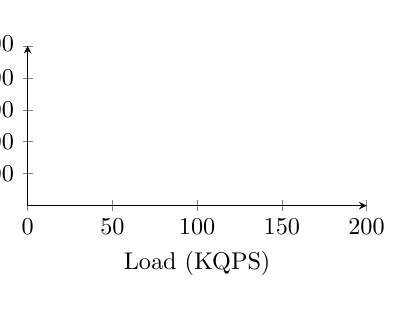
\begin{tikzpicture}[scale=0.875, transform shape, trim axis left, trim axis right]
                \begin{axis}[
                    \SyntheticHundredUsCommonAxis,
                    ylabel style={opacity=0},
                    ylabel={\phantom{Latency}},
                    legend style={
                        draw=none,
                        font=\footnotesize,
                        anchor=south,
                        at={(0.30, 1.10)},
                        legend columns=3,
                        /tikz/every even column/.append style={column sep=0.5cm},
                    },
                ]
                    \SyntheticHundredUsPlot{floatingStyle, x filter/.code={\IfStrEq{\thisrow{dist_config}}{exponential}{}{\def\pgfmathresult{}}}}{x expr=\thisrow{load_floating(QPS)} / 1000, y=latency_floating}{data/synthetic_80_100us.csv}
                    \SyntheticHundredUsPlot{workerPoolStyle, x filter/.code={\IfStrEq{\thisrow{dist_config}}{exponential}{}{\def\pgfmathresult{}}}}{x expr=\thisrow{load_pool(QPS)} / 1000, y=latency_pool}{data/synthetic_80_100us.csv}
                    \SyntheticHundredUsPlot{rakaiaStyle, x filter/.code={\IfStrEq{\thisrow{dist_config}}{exponential}{}{\def\pgfmathresult{}}}}{x expr=\thisrow{load_rakaia(QPS)} / 1000, y=latency_rakaia}{data/synthetic_80_100us.csv}
                    \SyntheticHundredUsPlot{partitionStyle, x filter/.code={\IfStrEq{\thisrow{dist_config}}{exponential}{}{\def\pgfmathresult{}}}}{x expr=\thisrow{load_partition(QPS)} / 1000, y=latency_partition}{data/synthetic_80_100us.csv}
                    \SyntheticHundredUsPlot{kcmStyle, x filter/.code={\IfStrEq{\thisrow{dist_config}}{exponential}{}{\def\pgfmathresult{}}}}{x expr=\thisrow{load_kcm_floating(QPS)} / 1000, y=latency_kcm_floating}{data/synthetic_80_100us.csv}
                    \SyntheticHundredUsSchedsimPlot{m}
                \end{axis}
            \end{tikzpicture}
            \caption{\add{Exponential (80 connections).}}
        \end{subfigure}
        \hfill
        \begin{subfigure}[b]{\SyntheticHundredUsPanelWidth}
            \centering
            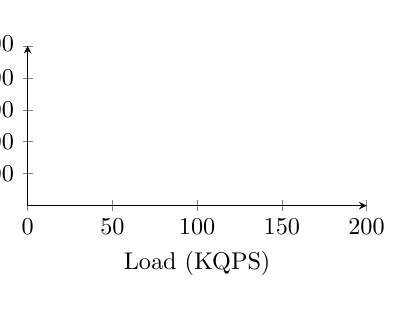
\begin{tikzpicture}[scale=0.875, transform shape, trim axis left, trim axis right]
                \begin{axis}[
                    \SyntheticHundredUsCommonAxis,
                    ylabel style={opacity=0},
                    ylabel={\phantom{Latency}},
                    legend style={
                        draw=none,
                        font=\footnotesize,
                        anchor=north east,
                        at={(0.40, 0.99)},
                    },
                ]
                    \SyntheticHundredUsPlot{floatingStyle, x filter/.code={\IfStrEq{\thisrow{dist_config}}{bimodal}{}{\def\pgfmathresult{}}}}{x expr=\thisrow{load_floating(QPS)} / 1000, y=latency_floating}{data/synthetic_80_100us.csv}
                    \SyntheticHundredUsPlot{workerPoolStyle, x filter/.code={\IfStrEq{\thisrow{dist_config}}{bimodal}{}{\def\pgfmathresult{}}}}{x expr=\thisrow{load_pool(QPS)} / 1000, y=latency_pool}{data/synthetic_80_100us.csv}
                    \SyntheticHundredUsPlot{rakaiaStyle, x filter/.code={\IfStrEq{\thisrow{dist_config}}{bimodal}{}{\def\pgfmathresult{}}}}{x expr=\thisrow{load_rakaia(QPS)} / 1000, y=latency_rakaia}{data/synthetic_80_100us.csv}
                    \SyntheticHundredUsPlot{partitionStyle, x filter/.code={\IfStrEq{\thisrow{dist_config}}{bimodal}{}{\def\pgfmathresult{}}}}{x expr=\thisrow{load_partition(QPS)} / 1000, y=latency_partition}{data/synthetic_80_100us.csv}
                    \SyntheticHundredUsPlot{kcmStyle, x filter/.code={\IfStrEq{\thisrow{dist_config}}{bimodal}{}{\def\pgfmathresult{}}}}{x expr=\thisrow{load_kcm_floating(QPS)} / 1000, y=latency_kcm_floating}{data/synthetic_80_100us.csv}
                    \SyntheticHundredUsSchedsimPlot{b}
                \end{axis}
            \end{tikzpicture}
            \caption{\add{Bimodal (80 connections).}}
        \end{subfigure}
    \end{minipage}

    \begin{minipage}{\linewidth}
        \centering
        \begin{subfigure}[b]{\SyntheticHundredUsPanelWidth}
            \centering
            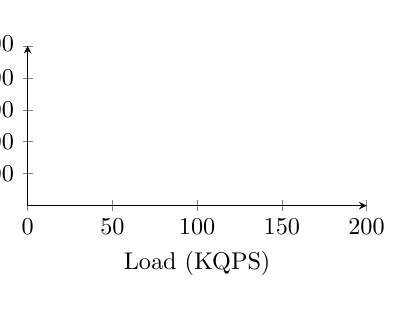
\begin{tikzpicture}[scale=0.875, transform shape, trim axis left, trim axis right]
                \begin{axis}[
                    \SyntheticHundredUsCommonAxis,
                    ylabel={Latency (\si{\micro\second})},
                    legend style={
                        draw=none,
                        font=\footnotesize,
                        anchor=south,
                        at={(0.90, 1.10)},
                        legend columns=3,
                        /tikz/every even column/.append style={column sep=0.7cm},
                    },
                ]
                    \SyntheticHundredUsPlot{partitionStyle, x filter/.code={\IfStrEq{\thisrow{dist_config}}{fixed}{}{\def\pgfmathresult{}}}}{x expr=\thisrow{load_partition(QPS)} / 1000, y=latency_partition}{data/synthetic_5000_100us.csv}
                    \SyntheticHundredUsPlot{floatingStyle, x filter/.code={\IfStrEq{\thisrow{dist_config}}{fixed}{}{\def\pgfmathresult{}}}}{x expr=\thisrow{load_floating(QPS)} / 1000, y=latency_floating}{data/synthetic_5000_100us.csv}
                    \SyntheticHundredUsPlot{workerPoolStyle, x filter/.code={\IfStrEq{\thisrow{dist_config}}{fixed}{}{\def\pgfmathresult{}}}}{x expr=\thisrow{load_pool(QPS)} / 1000, y=latency_pool}{data/synthetic_5000_100us.csv}
                    \SyntheticHundredUsPlot{kcmStyle, x filter/.code={\IfStrEq{\thisrow{dist_config}}{fixed}{}{\def\pgfmathresult{}}}}{x expr=\thisrow{load_kcm_floating(QPS)} / 1000, y=latency_kcm_floating}{data/synthetic_5000_100us.csv}
                    \SyntheticHundredUsPlot{rakaiaStyle, x filter/.code={\IfStrEq{\thisrow{dist_config}}{fixed}{}{\def\pgfmathresult{}}}}{x expr=\thisrow{load_rakaia(QPS)} / 1000, y=latency_rakaia}{data/synthetic_5000_100us.csv}
                    \SyntheticHundredUsSchedsimPlot{d}
                \end{axis}
            \end{tikzpicture}
            \caption{\add{Fixed (5{,}000 connections).}}
        \end{subfigure}
        \hfill
        \begin{subfigure}[b]{\SyntheticHundredUsPanelWidth}
            \centering
            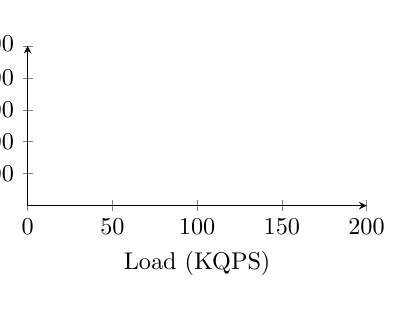
\begin{tikzpicture}[scale=0.875, transform shape, trim axis left, trim axis right]
                \begin{axis}[
                    \SyntheticHundredUsCommonAxis,
                    ylabel style={opacity=0},
                    ylabel={\phantom{Latency}},
                    legend style={
                        draw=none,
                        font=\footnotesize,
                        anchor=south,
                        at={(0.60, 1.10)},
                        legend columns=3,
                        /tikz/every even column/.append style={column sep=1cm},
                    },
                ]
                    \SyntheticHundredUsPlot{floatingStyle, x filter/.code={\IfStrEq{\thisrow{dist_config}}{exponential}{}{\def\pgfmathresult{}}}}{x expr=\thisrow{load_floating(QPS)} / 1000, y=latency_floating}{data/synthetic_5000_100us.csv}
                    \SyntheticHundredUsPlot{workerPoolStyle, x filter/.code={\IfStrEq{\thisrow{dist_config}}{exponential}{}{\def\pgfmathresult{}}}}{x expr=\thisrow{load_pool(QPS)} / 1000, y=latency_pool}{data/synthetic_5000_100us.csv}
                    \SyntheticHundredUsPlot{rakaiaStyle, x filter/.code={\IfStrEq{\thisrow{dist_config}}{exponential}{}{\def\pgfmathresult{}}}}{x expr=\thisrow{load_rakaia(QPS)} / 1000, y=latency_rakaia}{data/synthetic_5000_100us.csv}
                    \SyntheticHundredUsPlot{partitionStyle, x filter/.code={\IfStrEq{\thisrow{dist_config}}{exponential}{}{\def\pgfmathresult{}}}}{x expr=\thisrow{load_partition(QPS)} / 1000, y=latency_partition}{data/synthetic_5000_100us.csv}
                    \SyntheticHundredUsPlot{kcmStyle, x filter/.code={\IfStrEq{\thisrow{dist_config}}{exponential}{}{\def\pgfmathresult{}}}}{x expr=\thisrow{load_kcm_floating(QPS)} / 1000, y=latency_kcm_floating}{data/synthetic_5000_100us.csv}
                    \SyntheticHundredUsSchedsimPlot{m}
                \end{axis}
            \end{tikzpicture}
            \caption{\add{Exponential (5{,}000 connections).}}
        \end{subfigure}
        \hfill
        \begin{subfigure}[b]{\SyntheticHundredUsPanelWidth}
            \centering
            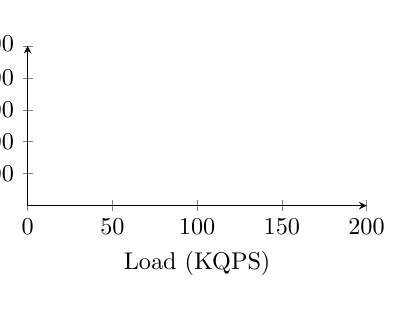
\begin{tikzpicture}[scale=0.875, transform shape, trim axis left, trim axis right]
                \begin{axis}[
                    \SyntheticHundredUsCommonAxis,
                    ylabel style={opacity=0},
                    ylabel={\phantom{Latency}},
                    legend style={
                        draw=none,
                        font=\footnotesize,
                        anchor=south,
                        at={(0.40, 1.10)},
                        legend columns=2,
                        /tikz/every even column/.append style={column sep=0.5cm},
                    },
                ]
                    \SyntheticHundredUsPlot{floatingStyle, x filter/.code={\IfStrEq{\thisrow{dist_config}}{bimodal}{}{\def\pgfmathresult{}}}}{x expr=\thisrow{load_floating(QPS)} / 1000, y=latency_floating}{data/synthetic_5000_100us.csv}
                    \SyntheticHundredUsPlot{workerPoolStyle, x filter/.code={\IfStrEq{\thisrow{dist_config}}{bimodal}{}{\def\pgfmathresult{}}}}{x expr=\thisrow{load_pool(QPS)} / 1000, y=latency_pool}{data/synthetic_5000_100us.csv}
                    \SyntheticHundredUsPlot{rakaiaStyle, x filter/.code={\IfStrEq{\thisrow{dist_config}}{bimodal}{}{\def\pgfmathresult{}}}}{x expr=\thisrow{load_rakaia(QPS)} / 1000, y=latency_rakaia}{data/synthetic_5000_100us.csv}
                    \SyntheticHundredUsPlot{partitionStyle, x filter/.code={\IfStrEq{\thisrow{dist_config}}{bimodal}{}{\def\pgfmathresult{}}}}{x expr=\thisrow{load_partition(QPS)} / 1000, y=latency_partition}{data/synthetic_5000_100us.csv}
                    \SyntheticHundredUsPlot{kcmStyle, x filter/.code={\IfStrEq{\thisrow{dist_config}}{bimodal}{}{\def\pgfmathresult{}}}}{x expr=\thisrow{load_kcm_floating(QPS)} / 1000, y=latency_kcm_floating}{data/synthetic_5000_100us.csv}
                    \SyntheticHundredUsSchedsimPlot{b}
                \end{axis}
            \end{tikzpicture}
            \caption{\add{Bimodal (5{,}000 connections).}}
        \end{subfigure}
    \end{minipage}
    \caption{\add{\nineninepct{} latency as a function of throughput for 100\si{\micro\second} tasks.
    Top, middle, and bottom rows correspond to 20, 80, and 5{,}000 client connections, respectively.}}\label{fig:synthetic_100us}
    \vspace{-0.5em}
\end{figure*}
